% =====================================================================
%  BLOCOS LaTeX PARA INSERÇÃO NO ARTIGO  (Lab04S03 — Suporte ao artigo)
%  Gerados a partir dos gráficos do dashboard (Sprints 1 e 2) e ajustados
%  à versão FINAL do artigo (main_aiddev.tex).
%
%  ── ANÁLISE DE ENCAIXE (onde cada gráfico agrega de fato) ────────────
%  • Seção 3 (Metodologia, \label{sec:method}): hoje só possui a figura do
%    pipeline (fig:pipeline) e NENHUMA figura descritiva do dataset. Os seis
%    blocos de caracterização abaixo são, portanto, adições genuínas e devem
%    entrar como uma nova \subsection ao final da Metodologia.
%  • Seção 4 (Resultados, \label{sec:results}):
%      – RQ01 (ccm_mean): o artigo JÁ possui a Figura~\ref{fig:ccm} (violino).
%        O box plot do dashboard é REDUNDANTE — incluído abaixo apenas como
%        ALTERNATIVA opcional (escolha um estilo: violino OU box plot).
%      – RQ02/RQ05 (design_smell_density): o artigo trata em TEXTO, SEM figura.
%        Este é o vazio real → a Figura~\ref{fig:dash-rq02} preenche a lacuna.
%
%  ── PADRÃO ADOTADO (consistente com o artigo) ───────────────────────
%  • Figuras: \begin{figure}[H] ... \includegraphics[width=.55\textwidth]{...}
%  • Tabelas: \begin{adjustbox}{max width=\textwidth}\small ... \end{adjustbox}
%  • Vírgula decimal via $0{,}xxx$; percentuais com \,\%; variáveis em \texttt{}.
%  • Preâmbulo já presente no artigo: graphicx, booktabs, adjustbox, float.
%
%  ── COMO USAR ───────────────────────────────────────────────────────
%  1. Exporte cada gráfico do dashboard como PNG e salve NESTA pasta
%     (mesma de main_aiddev.tex e dos violinos) com o nome de \includegraphics.
%  2. Cole os parágrafos + ambientes na seção indicada.
%  3. Todos os números abaixo foram apurados sobre o dataset real
%     (N = 202.014 PRs; 1.290 repositórios; G1 = IA, n = 9; G2 = humano,
%     n = 202.005) e conferidos célula a célula contra dataset_final.csv.
% =====================================================================


% #####################################################################
% ###  SEÇÃO 3 (METODOLOGIA) — inserir como nova \subsection ao final  ###
% ###  da Seção~\ref{sec:method}, antes da Seção de Resultados.        ###
% #####################################################################

\subsection{Caracterização do Dataset}
\label{sec:caracterizacao}

Antes da inferência por questão de pesquisa, caracteriza-se a composição e a
tendência central das variáveis de processo do dataset de análise, de modo a
contextualizar a forte assimetria amostral entre os grupos e a natureza
enviesada das distribuições. O conjunto reúne 202.014 Pull Requests merged
distribuídos em 1.290 repositórios populares, particionados no Grupo IA (G1,
n = 9) e no Grupo Humano (G2, n = 202.005). Como as variáveis contínuas são
acentuadamente assimétricas e de cauda longa, adota-se a \textbf{mediana} como
medida de tendência central de referência, reportando-se a média e o intervalo
interquartil (IQR) como apoio --- decisão que fundamenta o uso de testes não
paramétricos descrito na Seção~\ref{sec:results}.

% --------------------------------------------------------------------
%  Figura: distribuição por linguagem
% --------------------------------------------------------------------
A Figura~\ref{fig:dash-linguagem} apresenta a distribuição dos PRs pelas três
linguagens consideradas. O dataset é dominado por TypeScript, com 98.520 PRs
(48,8\,\%), seguido de Python, com 65.868 PRs (32,6\,\%), e JavaScript, com
37.626 PRs (18,6\,\%). Essa predominância de TypeScript em G2 contrasta com a
composição de G1 --- majoritariamente Python (8 de 9 PRs) ---, o que antecipa
a única diferença estatisticamente robusta observada no estudo (distribuição
de \texttt{language}; ver Tabela~\ref{tab:resumo}) e reforça que tal diferença
é um artefato de composição amostral, e não um indicador de manutenibilidade.

\begin{figure}[H]
\centering
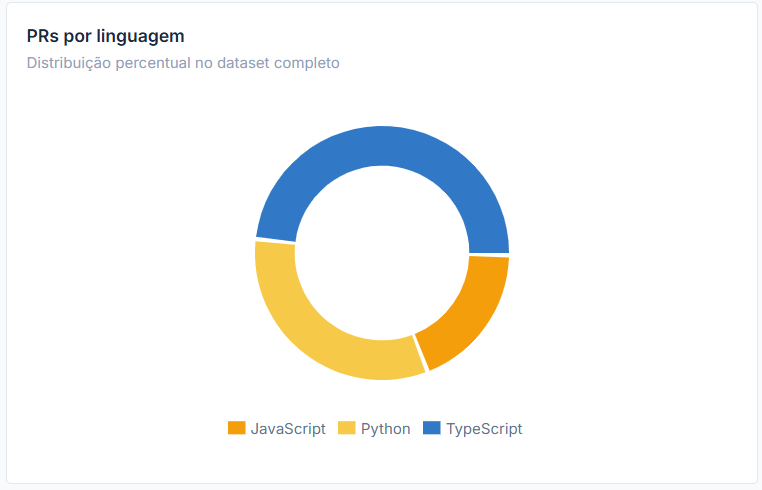
\includegraphics[width=.6\textwidth]{dashboard_dist_linguagem.png}
\caption{Distribuição dos PRs por linguagem de programação no dataset de
análise (N = 202.014). TypeScript concentra 48,8\,\% das contribuições.}
\label{fig:dash-linguagem}
\end{figure}

% --------------------------------------------------------------------
%  Figura: distribuição por agente (fingerprint)
% --------------------------------------------------------------------
A Figura~\ref{fig:dash-agente} detalha a procedência das contribuições segundo
o \textit{fingerprint} comportamental \cite{ghaleb:26} do agente de IA
associado ao PR. Devin responde pela maior parcela, com 134.718 PRs
(66,7\,\%), seguido de Claude Code, com 24.769 PRs (12,3\,\%), Cursor, com
3.696 PRs (1,8\,\%), e OpenAI Codex, com 7 PRs ($\approx$\,0,0\,\%); 38.824 PRs
(19,2\,\%) não receberam atribuição de \textit{fingerprint}. Cabe destacar que
essa identificação opera sobre todo o dataset --- inclusive sobre PRs de G2 ---
porque o \textit{fingerprint} sinaliza o ferramental de IA empregado em
contribuições assistidas e confirmadas por humanos, e não apenas as
contribuições plenamente autônomas que compõem G1.

\begin{figure}[H]
\centering
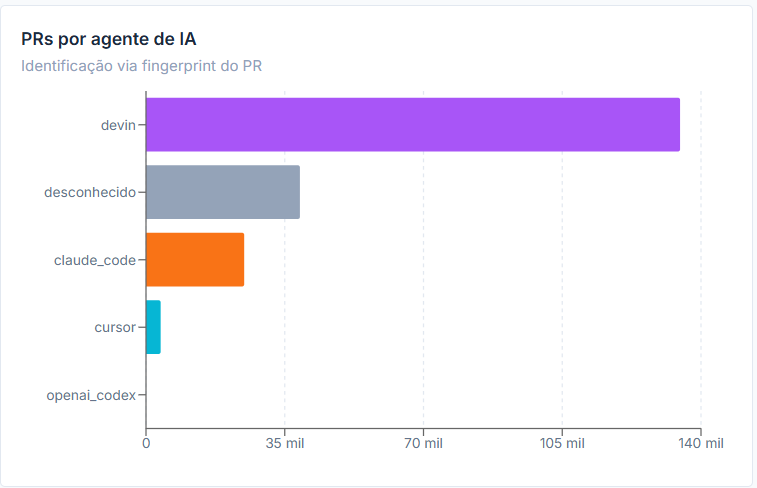
\includegraphics[width=.7\textwidth]{dashboard_dist_agente.png}
\caption{Distribuição dos PRs por agente de IA identificado via
\textit{fingerprint} comportamental \cite{ghaleb:26}. Devin concentra
66,7\,\% das contribuições atribuídas; 19,2\,\% ficam sem atribuição.}
\label{fig:dash-agente}
\end{figure}

% --------------------------------------------------------------------
%  Tabela: tendência central das métricas de processo
% --------------------------------------------------------------------
A Tabela~\ref{tab:dash-central} sumariza a tendência central das principais
variáveis de processo. O contraste sistemático entre mediana e média evidencia
a assimetria positiva das distribuições: em \texttt{diff\_lines}, por exemplo,
a mediana de 71 linhas é muito inferior à média de 119, revelando uma cauda
longa de PRs grandes. O tempo até o merge é tipicamente curto (mediana de
0,62 dia), porém com média de 4,34 dias puxada por \textit{outliers}. A baixa
proporção mediana de arquivos de teste (0; média 0,18) e a presença de revisão
formal em 73,5\,\% dos PRs (\texttt{has\_review}; cf.\ Tabela~\ref{tab:hasreview})
caracterizam o processo de contribuição predominante.

\begin{table}[H]
\centering
\caption{Tendência central das métricas de processo (dataset de análise,
N = 202.014). IQR = intervalo interquartil [P25; P75].}
\label{tab:dash-central}
\begin{adjustbox}{max width=\textwidth}
\small
\begin{tabular}{lrrr}
\toprule
\textbf{Métrica} & \textbf{Mediana} & \textbf{Média} & \textbf{IQR [P25; P75]} \\
\midrule
Linhas alteradas (\texttt{diff\_lines})          & 71   & 118,99 & [28; 172] \\
Arquivos alterados (\texttt{changed\_files})     & 4    & 6,32   & [2; 7] \\
Tempo até o merge (\texttt{days\_to\_merge})     & 0,62 & 4,34   & [0,05; 2,79] \\
Commits por PR (\texttt{commit\_count})          & 3    & 3,70   & [1; 5] \\
Revisões por PR (\texttt{review\_count})         & 1    & 2,32   & [0; 3] \\
Prop.\ arq.\ de teste (\texttt{test\_file\_ratio}) & 0  & 0,18   & [0; 0,33] \\
\bottomrule
\end{tabular}
\end{adjustbox}
\end{table}

% --------------------------------------------------------------------
%  Figura: histograma de diff_lines
% --------------------------------------------------------------------
A Figura~\ref{fig:dash-diffhist} mostra o histograma de \texttt{diff\_lines}.
A massa da distribuição concentra-se em PRs pequenos a médios --- a faixa de
0--100 linhas reúne a maioria das contribuições ---, com decaimento acentuado
e cauda longa à direita. Esse formato justifica metodologicamente o emprego de
testes não paramétricos (Mann-Whitney U) e da mediana como medida-síntese, em
detrimento da média, sensível aos \textit{outliers}.

\begin{figure}[H]
\centering
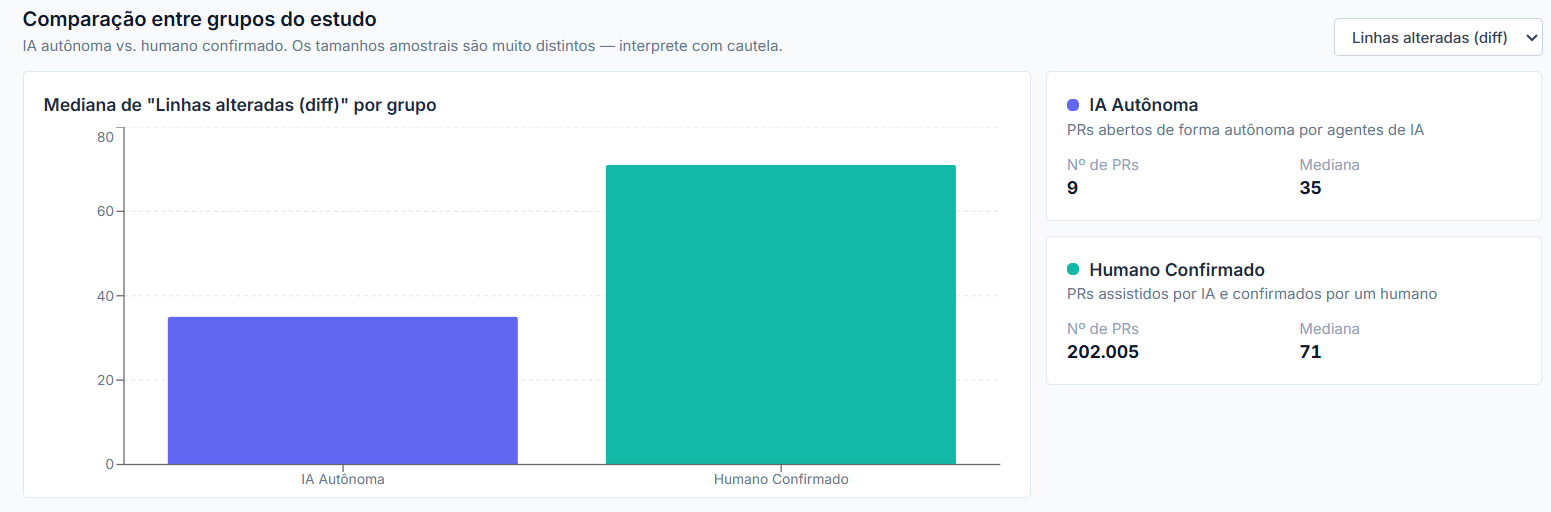
\includegraphics[width=.7\textwidth]{dashboard_hist_diff.png}
\caption{Histograma do número de linhas alteradas por PR (\texttt{diff\_lines}).
Eixo Y: nº de PRs; eixo X: faixas de linhas no diff. Forte assimetria positiva
com cauda longa à direita.}
\label{fig:dash-diffhist}
\end{figure}

% --------------------------------------------------------------------
%  Figura: histograma de days_to_merge
% --------------------------------------------------------------------
A Figura~\ref{fig:dash-dias} apresenta o histograma de \texttt{days\_to\_merge}.
A grande maioria dos PRs é integrada em menos de um dia, refletindo um fluxo de
revisão e merge ágil; ainda assim, observa-se uma cauda de PRs que permanecem
abertos por semanas, responsável pela discrepância entre a mediana (0,62 dia) e
a média (4,34 dias) reportadas na Tabela~\ref{tab:dash-central}.

\begin{figure}[H]
\centering
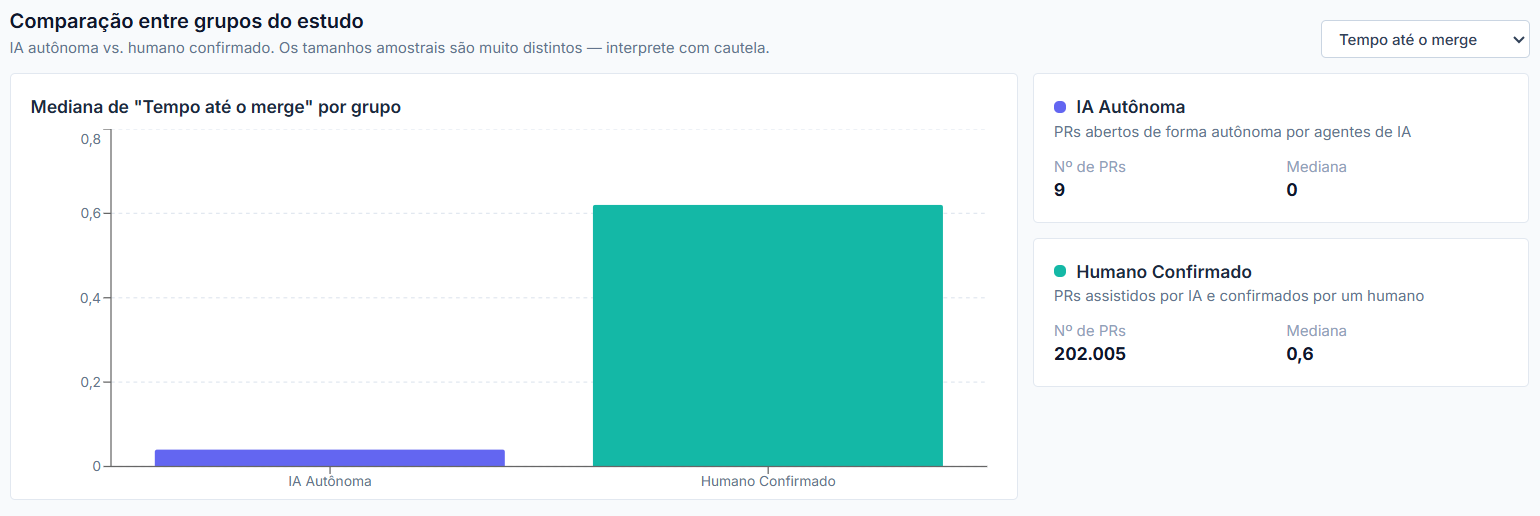
\includegraphics[width=.7\textwidth]{dashboard_hist_dias.png}
\caption{Histograma do tempo até o merge (\texttt{days\_to\_merge}).
Eixo Y: nº de PRs; eixo X: faixas de dias. Predomínio de merges em menos de
um dia.}
\label{fig:dash-dias}
\end{figure}

% --------------------------------------------------------------------
%  Figura: diff por linguagem (controle de confusão por subgrupo)
% --------------------------------------------------------------------
Por fim, a Figura~\ref{fig:dash-difflang} compara a tendência central de
\texttt{diff\_lines} entre as três linguagens. As medianas são notavelmente
homogêneas --- 70 linhas em TypeScript, 73 em Python e 69 em JavaScript ---,
indicando que o tamanho típico das contribuições não varia de forma relevante
entre as linguagens e que a linguagem, isoladamente, não constitui fator de
confusão para o tamanho dos PRs.

\begin{figure}[H]
\centering
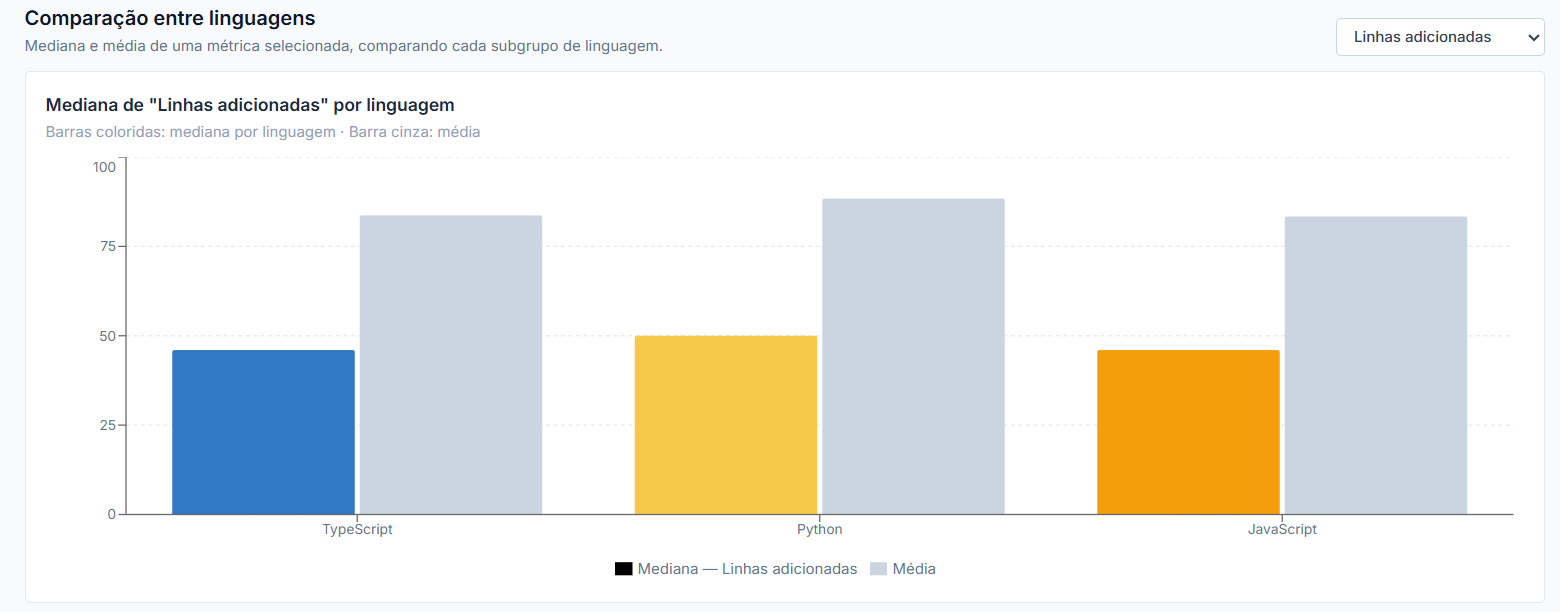
\includegraphics[width=.7\textwidth]{dashboard_diff_por_linguagem.png}
\caption{Mediana e média de \texttt{diff\_lines} por linguagem. As medianas
($\approx$ 70 linhas) são homogêneas entre os subgrupos, afastando a linguagem
como fator de confusão para o tamanho das contribuições.}
\label{fig:dash-difflang}
\end{figure}


% #####################################################################
% ###  SEÇÃO 4 (RESULTADOS) — inserir em Seção~\ref{sec:results}       ###
% #####################################################################

% --------------------------------------------------------------------
%  RQ02 / RQ05 — Densidade de Code Smells de Design / KLoC
%  >>> ADIÇÃO RECOMENDADA: o artigo discute esta métrica em TEXTO e NÃO
%      possui figura para ela. Esta figura preenche essa lacuna.
%      Sugestão: inserir na subseção "Q3: Dívida Técnica Estrutural",
%      logo após o parágrafo de RQ05.
% --------------------------------------------------------------------
A Figura~\ref{fig:dash-rq02} ilustra a distribuição da densidade de
\textit{code smells} de design por KLoC (\texttt{design\_smell\_density}) entre
os grupos (n = 9 em G1; n = 50 em G2), por meio de um \textit{box plot} com os
pontos individuais sobrepostos. Em ambos os grupos a \textbf{mediana é igual a
zero}: a maioria dos PRs não acusa \textit{smells} de design. As poucas
observações positivas --- uma em G1 ($\approx$ 5,52) e três em G2 ($\approx$
3,61, 6,10 e 8,03) --- são \textit{outliers} que não deslocam a tendência
central. Coerentemente, o teste de Mann-Whitney U não indicou diferença
estatisticamente significativa ($p = 0{,}612$; Cliff's $\delta = 0{,}049$,
negligível), conforme já reportado para RQ05. \textbf{H0 não é rejeitada}
($\alpha = 0{,}05$).

\begin{figure}[H]
\centering
\includegraphics[width=.55\textwidth]{dashboard_rq02_smells.png}
\caption{RQ02/RQ05 --- Distribuição da densidade de \textit{code smells} de
design por KLoC (\texttt{design\_smell\_density}) por grupo (n = 9 G1; n = 50
G2). Mediana igual a zero em ambos; diferença não significativa ($p = 0{,}612$;
$\delta = 0{,}049$). \textit{Proxy} via Lizard (funções longas, NLOC $>$ 50),
sem ESLint/Pylint.}
\label{fig:dash-rq02}
\end{figure}

% --------------------------------------------------------------------
%  RQ01 — CCM  (OPCIONAL / ALTERNATIVA)
%  >>> O artigo JÁ possui a Figura~\ref{fig:ccm} (violino). Use o bloco
%      abaixo APENAS se quiser trocar o violino pelo box plot do dashboard
%      (escolha UM estilo para manter consistência visual). Caso mantenha
%      o violino, DESCARTE este bloco.
% --------------------------------------------------------------------
\iffalse  % <- remova este \iffalse ... \fi para ativar o bloco
A Figura~\ref{fig:dash-rq01} apresenta, de forma alternativa à
Figura~\ref{fig:ccm}, a distribuição da complexidade ciclomática média
(\texttt{ccm\_mean}; \cite{mccabe:76}) por grupo (n = 3 em G1; n = 32 em G2)
em um \textit{box plot} com pontos sobrepostos. A mediana de G1 ($\approx$
5,38) é substancialmente mais alta do que a de G2 ($\approx$ 1,25), com
tamanho de efeito grande (Cliff's $\delta = 0{,}71$); contudo, o $p$ bruto de
0,043 não sobrevive à correção para múltiplos testes ($p_{\text{BH}} = 0{,}142$),
e o n mínimo de G1 reduz o achado a indício exploratório. \textbf{H0 não é
rejeitada} ($\alpha = 0{,}05$).

\begin{figure}[H]
\centering
\includegraphics[width=.55\textwidth]{dashboard_rq01_ccm.png}
\caption{RQ01 --- Distribuição de \texttt{ccm\_mean} por grupo (n = 3 G1;
n = 32 G2), em \textit{box plot}. G1 exibe mediana mais alta ($\approx$ 5,38)
que G2 ($\approx$ 1,25); sem significância após correção.}
\label{fig:dash-rq01}
\end{figure}
\fi
